%%%%%%%%%%%%%%%%%%%%%%%%%%%%%%%%%%%%%%%%%%%%%%%%%%%%%%%%%%%%%%%%%%%%
%% I, the copyright holder of this work, release this work into the
%% public domain. This applies worldwide. In some countries this may
%% not be legally possible; if so: I grant anyone the right to use
%% this work for any purpose, without any conditions, unless such
%% conditions are required by law.
%%%%%%%%%%%%%%%%%%%%%%%%%%%%%%%%%%%%%%%%%%%%%%%%%%%%%%%%%%%%%%%%%%%%

\documentclass{beamer}
\usetheme[faculty=phil]{fibeamer}
\usepackage[utf8]{inputenc}
\usepackage[
  main=english, %% By using `czech` or `slovak` as the main locale
                %% instead of `english`, you can typeset the
                %% presentation in either Czech or Slovak,
                %% respectively.
  czech, slovak %% The additional keys allow foreign texts to be
]{babel}        %% typeset as follows:
%%
%%   \begin{otherlanguage}{czech}   ... \end{otherlanguage}
%%   \begin{otherlanguage}{slovak}  ... \end{otherlanguage}
%%
%% These macros specify information about the presentation
\title{Classical Black Holes} %% that will be typeset on the
\subtitle{02. Black holes Introduction} %% title page.
\author{Edward Larra\~{n}aga}
%% These additional packages are used within the document:
\usepackage{ragged2e}  % `\justifying` text
\usepackage{booktabs}  % Tables
\usepackage{tabularx}
\usepackage{tikz}      % Diagrams
\usetikzlibrary{calc, shapes, backgrounds}
\usepackage{amsmath, amssymb}
\usepackage{url}       % `\url`s
\usepackage{listings}  % Code listings
\usepackage{siunitx}
\frenchspacing
\begin{document}
  \frame{\maketitle}

  \AtBeginSection[]{% Print an outline at the beginning of sections
    \begin{frame}<beamer>
      \frametitle{Outline for Part \thesection}
      \tableofcontents[currentsection]
    \end{frame}}
    \section{Black Holes Introduction}
    
    \subsection{Newtonian Gravity}
    	\begin{frame}{Newton's Law of Gravity}
			$$ \vec{F} = - \frac{G M m }{r^{2}} \hat{r}$$  
       		$$ G = 6.67 \times 10 ^{-11} \frac{\mathrm{N \cdot m^{2}}}{\mathrm{kg^{2}}} $$  
    	\end{frame}
        
        \begin{frame}{Escape Velocity}
        	$$ v_{esc} = \sqrt[]{\frac{2GM}{r}} $$
        \end{frame}
        
        \begin{frame}{Schwarzschild's Radius}
        	$$ r_S = \frac{2GM}{c^2} $$
        \end{frame}
        
        \begin{frame}{Schwarzschild's Radius}
        	\begin{center}
        		\begin{tabular}{c | c | c}
          		\textbf{Object}	& \textbf{Mass} ($M_\odot\ $) & \textbf{Schwarzschild's Radius} (\si{km})\\
          		\hline
          		Earth & $ 3 \times 10^{-6} $	& $8.9 \times 10^{-6}$\\ 
          		Sun 	& $ 1 $	& $2.95$                 
        		\end{tabular}    
    		\end{center}	
        \end{frame}
        
        \begin{frame}{Critical Density for the formation of a Black Hole}
        	$$ \rho_c = \frac{M}{\frac{4 \pi r_s^3}{3}}$$
            \pause
            $$ \rho_c = \frac{3c^6}{32 \pi G^3 M^2}$$
			\pause
            $$ \rho_c \sim 10^{19} \si{kg \per m^3} \sim 10^{16} \si{g \per cm^3} $$
        \end{frame}
        
        \subsection{Important Advances in the XX Century}
        \begin{frame}{Important Advances in the XX Century}
        	\begin{itemize}
        	\item General Relativity (Relativistic Theory of Gravity)
            \pause
            \item Schwarzschild's Solution (1916)
            \pause
            \item Gravitational Collapse of stellar objects description (1920's) 
            \pause
            \item Discovery of matter with densities in the range $10^9$ to $10^{17} \si{kg \per m^3}$.\\
            White Dwarfs and Neutron Stars (1930's - 1950's)
            \pause
            \item Evidence of supermassive (and superdense) objects in AGN's (1960's - 1970's)
        	\end{itemize}      
        \end{frame}
        
        \subsection{{Top Reasons to Study Black Holes}}
        \begin{frame}{Top Reasons to Study Black Holes}
        	\begin{itemize}
        	\item To understand strong gravitational fields.
           	\pause
            \item To understand the final stages of stellar evolution.
            \pause
            \item Potential insight of the connection between quantum physics and gravity.
            \pause
            \item Potential insight of the connection between thermodynamics and gravity.
        	\end{itemize}
        \end{frame}
        
      


  	\section{Schwarzschild's Black Hole}
  	\begin{darkframes}
  
    	\subsection{General Relativity Field Equations}

    	\begin{frame}{Einstein Field Equations}
    		Einstein field equations are 
			$$ G_{\mu\nu} = R_{\mu\nu} - \frac{1}{2}g_{\mu\nu}R = 8\pi GT_{\mu\nu} $$
        	\pause
        	$$ G_{\mu\nu} = R_{\mu\nu} - \frac{1}{2}g_{\mu\nu}R $$
    	\end{frame}
        
    	\begin{frame}{Riemann Tensor}
    		Riemann tensor is defined as
			$$ R_{\;\mu\rho\nu}^{\lambda} = 
            \partial_{\rho}\Gamma_{\nu\mu}^{\lambda}-	
            \partial_{\nu}\Gamma_{\rho\mu}^{\lambda}+ 
            \Gamma_{\rho\alpha}^{\lambda}\Gamma_{\nu\mu}^{\alpha}-
            \Gamma_{\nu\alpha}^{\lambda}\Gamma_{\rho\mu}^{\alpha}$$  
            \pause
            $$ \Gamma^{\nu}_{\mu \sigma} = \frac{1}{2} g^{\nu \alpha} \left[ 
            \partial_{\mu} g_{\alpha \sigma} + 
            \partial_{\sigma} g_{\mu \alpha} - 
            \partial_{\alpha} g_{\mu \sigma} \right] $$
    	\end{frame}

		\begin{frame}{Ricci Tensor and Curvature Scalar}	
			$$R_{\mu\nu}=g^{\sigma\rho}R_{\sigma\mu\rho\nu}$$
    		$$R = R_{\sigma}^{\sigma} = g^{\sigma\tau}R_{\sigma\tau}. $$
    	\end{frame}
        
        \begin{frame}{Ricci Tensor and Curvature Scalar}	
			$$R_{\mu\nu}=\partial_{\rho}\Gamma_{\nu\mu}^{\rho}-	
            \partial_{\nu}\Gamma_{\rho\mu}^{\rho}+ 
            \Gamma_{\rho\alpha}^{\rho}\Gamma_{\nu\mu}^{\alpha}-
            \Gamma_{\nu\alpha}^{\rho}\Gamma_{\rho\mu}^{\alpha}$$
            
    		$$R = g^{\sigma\tau}\partial_{\rho}\Gamma_{\tau\sigma}^{\rho}-	
            g^{\sigma\tau}\partial_{\tau}\Gamma_{\rho\sigma}^{\rho}+ 
            g^{\sigma\tau}\Gamma_{\rho\alpha}^{\rho}\Gamma_{\tau\sigma}^{\alpha}-
            g^{\sigma\tau}\Gamma_{\tau\alpha}^{\rho}\Gamma_{\rho\sigma}^{\alpha}$$
    	\end{frame}
    	
        \begin{frame}{Einstein Field Equations}
			$$ R_{\mu\nu} - \frac{1}{2}g_{\mu\nu}R = 8\pi GT_{\mu\nu} $$
        	\pause
            \small{
			\begin{align*}
	            &\partial_{\rho}\Gamma_{\nu\mu}^{\rho}-	
    	        \partial_{\nu}\Gamma_{\rho\mu}^{\rho}+ 
        	    \Gamma_{\rho\alpha}^{\rho}\Gamma_{\nu\mu}^{\alpha}-
            	\Gamma_{\nu\alpha}^{\rho}\Gamma_{\rho\mu}^{\alpha} \\
            	&-\frac{1}{2}g_{\mu\nu} \left[ 
            	g^{\sigma\tau}\partial_{\rho}\Gamma_{\tau\sigma}^{\rho}- 	
            	g^{\sigma\tau}\partial_{\tau}\Gamma_{\rho\sigma}^{\rho}+  
            g^{\sigma\tau}\Gamma_{\rho\alpha}^{\rho}\Gamma_{\tau\sigma}^{\alpha}- 
            	g^{\sigma\tau}\Gamma_{\tau\alpha}^{\rho}\Gamma_{\rho\sigma}^{\alpha} 
            	\right] = 8\pi G T_{\mu\nu} 
            \end{align*} }
    	\end{frame}
       	
        \subsection{Physical Conditions to obtain Schwarzschild's Metric}
        \begin{frame}{Physical Conditions to obtain Schwarzschild's Metric}
        	\begin{itemize}
        	\item Spherical Symmetry
            \pause
            \item Asymptotically flat spacetime
            \pause
            \item Static Metric
            \pause
            \item Empty Spacetime
        	\end{itemize}
        \end{frame}
		
        \begin{frame}{Physical Conditions to obtain Schwarzschild's Metric}
        	\begin{itemize}
        	\item Spherical Symmetry
            \end{itemize}
			\pause
            Spherical Coordinates: $(t, r, \theta, \phi)$
            \pause
            \bigskip
            
            $$ ds^2 = - g_{tt} dt^2 + g_{rr} dr^2 + g_{\theta\theta} d\theta^2 + g_{\phi\phi} d\phi^2 $$
            \pause
            \bigskip
            $$ ds^2 = - g_{tt} dt^2 + g_{rr} dr^2 + r^2 d\theta^2 + r^2 \sin^2 \theta d\phi^2 $$
            \pause
            \begin{align*}
            g_{tt} &= g_{tt} (t,r)\\
            g_{rr} &= g_{rr} (t,r)
            \end{align*}
        \end{frame}
        
        \begin{frame}{Physical Conditions to obtain Schwarzschild's Metric}
        	\begin{itemize}
            \item Asymptotically flat
            \pause
            \begin{align*}
            \lim_{r \rightarrow \infty} g_{tt} &\longrightarrow 1 \\
            \lim_{r \rightarrow \infty} g_{rr} &\longrightarrow 1
            \end{align*}
        	\end{itemize}
        \end{frame}
        
        \begin{frame}{Physical Conditions to obtain Schwarzschild's Metric}
        	\begin{itemize}
            \item Static Metric
        	\end{itemize}
            \pause
            \begin{align*}
            g_{tt} &= g_{tt} (r)\\
            g_{rr} &= g_{rr} (r)
            \end{align*}
            \pause
            \centering
            {"Birkhoff Theorem"}
        \end{frame}
        
        \begin{frame}{Physical Conditions to obtain Schwarzschild's Metric}
        	\begin{itemize}
            \item Empty Spacetime
        	\end{itemize}
            \pause
            $$ T_{\mu\nu} = 0 $$
            \pause
            \bigskip
            Field Equations:
            $$ R_{\mu\nu} = 0 $$
        \end{frame}
        
    \subsection{Schwarzschild's Solution}
    	\begin{frame}{Schwarzschild's Solution}
    		$$ ds^2 = - \left( 1 - \frac{2GM}{c^2 r} \right) dt^2 
            + \left( 1 - \frac{2GM}{c^2 r} \right)^{-1} dr^2 
            + r^2 d\theta^2 + r^2 \sin^2 \theta d\phi^2 $$
            \pause
            \bigskip
            
            $M$: Mass associated to the black hole \\
            (Total energy content in spacetime)
    	\end{frame}
	
    	\begin{frame}{Schwarzschild's Solution}
    		$$ ds^2 = - \left( 1 - \frac{2M}{r} \right) dt^2 
            + \left( 1 - \frac{2M}{r} \right)^{-1} dr^2 
            + r^2 d\Omega^{2} $$
            \pause
            $$ d\Omega^{2} = d\theta^2 + \sin^2 \theta d\phi^2 $$
            \bigskip
            
            Geometrical units: $ G = c = 1$ 
    	\end{frame}
        
        \subsection{Physical Properties of Schwarzschild's Solution}
    	\begin{frame}{Physical Properties of Schwarzschild's Solution}
    		The limit $r \rightarrow \infty $ gives Minkowski's metric,
            $$ ds^{2}=-dt^{2}+dr^{2}+r^{2}d\Omega^{2}. $$
            \pause
            \centering
            {Asymptotically flat spacetime}
    	\end{frame}
        
        \begin{frame}{Interpretation of Coordinates in Schwarzschild's Solution}
			1. If we consider a surface with $t = constant $ and $r = R = constant$, i.e. such that $dt = dr = 0$, the remaining terms in the line element are	
			$$ ds^2 = R^2 d\Omega^2 = R^2 \left( d\theta^2 + \sin^{2} \theta d\phi^2 \right),$$
which corresponds to the measure of length on the surface of a sphere
of radius $R$.\\ 
\textit{We interpret $\left(\theta,\phi\right)$
as the usual spherical angular coordinates.}
    	\end{frame}
        
        \begin{frame}{Interpretation of Coordinates in Schwarzschild's Solution}
			2. Consider a static observer at the coordinates	$\left( r, \theta, \phi \right) = \left( R, \theta_0, \phi_0 \right)$, i.e. with $dr = d\theta = d\varphi = 0$.\\

The line element becomes
$$ ds^2 = -\left( 1 - \frac{2M}{R} \right) dt^2 $$
or in terms of the proper time $\tau_{R}$ of the static observer
at radius $R$,
$$ d\tau_R^2=\left( 1 - \frac{2M}{R} \right) dt^2. $$
    	\end{frame}
        
        \begin{frame}{Interpretation of Coordinates in Schwarzschild's Solution}
        	\begin{itemize}
        	\item Now consider a static observer located at the asymptotic region, $R \longrightarrow \infty$. \textit{The coordinate time $t$ corresponds to the proper time of the static asymptotic observer,}
$$ d\tau_\infty ^2 = dt^2 .$$
			\pause
			The proper time $d\tau_R$ runs slower that the asymptotic time $dt$ by the \textit{gravitational redshift factor} $\sqrt{1-\frac{2M}{R}}$.\\
            \pause
            \bigskip
			\item For $R \longrightarrow 2M$, we have $d\tau_R \longrightarrow 0$.
          	\end{itemize}
    	\end{frame}
        
        \begin{frame}{Interpretation of Coordinates in Schwarzschild's Solution}
        	3. To consider radial proper distance, let $ dt = d\theta = d\phi = 0 $ in the line element. The
\textit{proper radial length} is given by the differential quantity $dl$,
$$ ds^2 = dl^2 = \left( 1 - \frac{2M}{r} \right)^{-1} dr^2 $$
			\pause
            \textit{A ruler located radially in this spacetime measures $dl$ and not $dr$}.
    	\end{frame}
        
        \begin{frame}{Gravitational Redshift}
        	The wavelength of an electromagnetic wave is proportional to its period, $\tau=\frac{\lambda}{c}$.\\
            \bigskip
            The relation between the wavelength $\lambda$ as seen by an static observer at radius $R$ and the wavelength $\lambda_{\infty}$ as seen by an asymptotic static observer is
$$ \lambda = \sqrt{ 1 - \frac{2M}{R}} \lambda_\infty $$
        \end{frame}
        
        \begin{frame}{Gravitational Redshift}
        	The redshift factor $z$ is defined as
			$$ z = \frac{ \lambda_\infty - \lambda}{\lambda} $$
			from which 
			$$ 1 + z = 
            \left( 1 - \frac{2M}{R} \right)^{-\frac{1}{2}} $$
        \end{frame}
        
        \begin{frame}{Physical Properties of Schwarzschild's Solution}
    		Singularities
            \begin{itemize}
				\item $r = 0$ 
				\item $r = 2M$ 
            \end{itemize}
    	\end{frame}
        
        \begin{frame}{Physical Properties of Schwarzschild's Solution}
    		Singularities
            \begin{itemize}
				\item $r = 0$ \\
                \pause
                Essential Singularity
            \end{itemize}
            \pause
            \bigskip
            
            $$ K = R_{\alpha\beta\mu\nu} R^{\alpha\beta\mu\nu} = \frac{48M^{2}}{r^{6}}$$
            \centering
            {Kretchmann Scalar}
    	\end{frame}
        
        \begin{frame}{Physical Properties of Schwarzschild's Solution}
    		Singularities
            \begin{itemize}
				\item $r = 2M$  : Schwarzschild's radius\\
                \pause
                Coordinate Singularity
            \end{itemize}
            \pause
            \bigskip
            
            The infinite value of the line element at this value can be
removed with a change of coordinates (e.g. Eddington-Finkelstein
coordinates)
    	\end{frame}
        
        \begin{frame}{Causal Structure of Schwarzschild's Metric}
            Ingoing radial light rays move according to the conditions
            \begin{align*}
            	ds^2 &= 0\\ 
            	d\Omega &= 0
            \end{align*}
            \pause
            \bigskip
            
            $$ \frac{dt}{dr}=\pm\frac{1}{\left(1-\frac{2M}{r}\right)} $$
    	\end{frame}
  
  \end{darkframes}        
        \begin{frame}{Causal Structure of Schwarzschild's Metric}
        	\begin{center}
				\begin{figure}
%\begin{center}
				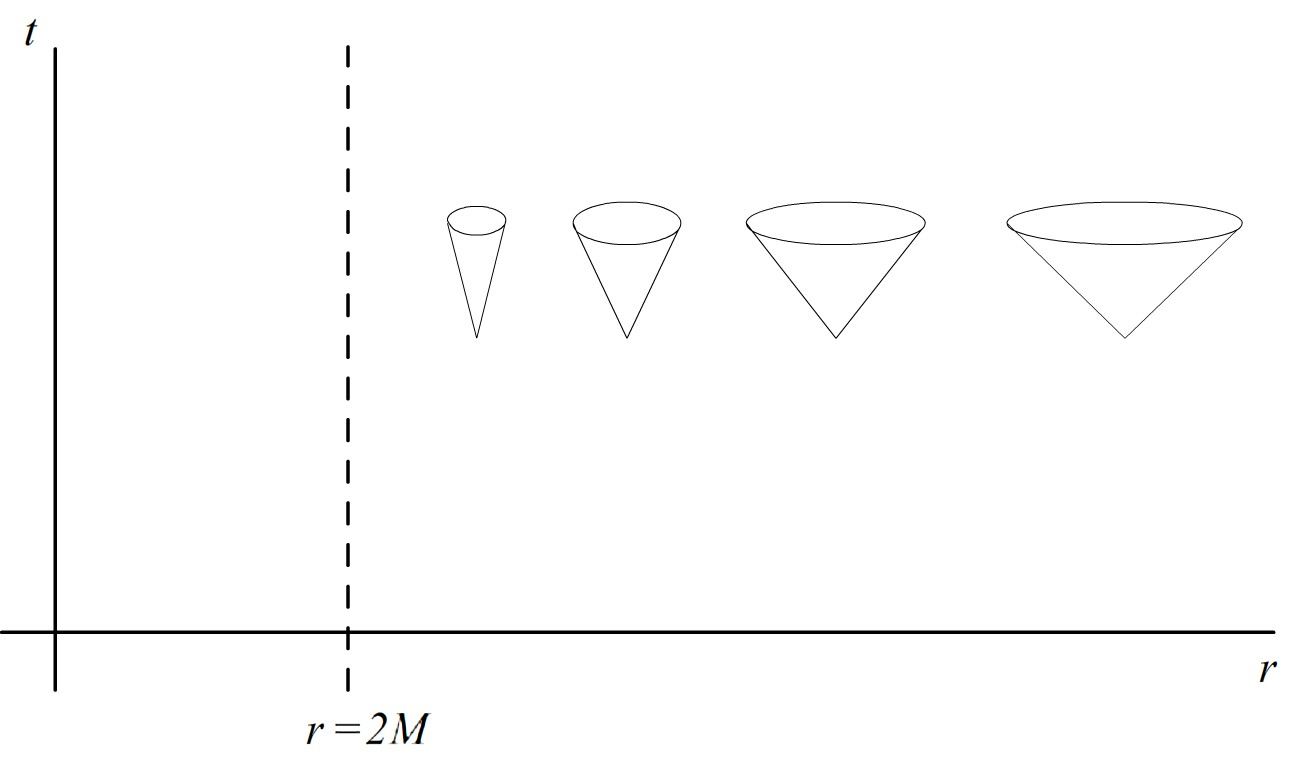
\includegraphics[scale=0.75]	{fig1.jpg}
%\end{center}
				\end{figure}
                \tiny{
                $$ \frac{dt}{dr}=\pm\frac{1}{\left(1-\frac{2M}{r}\right)} $$}
			\end{center}
        \end{frame}

  
  \begin{darkframes}
        \begin{frame}{Killing Vector Fields}
			$\xi = \frac{\partial}{\partial t}$\\
            \pause
            - Timelike for $r>2M$\\
            \pause
            - Temporal Inversion Symmetry\\
            \pause
            \bigskip
            
			$\zeta = \frac{\partial}{\partial\phi}$\\
            \pause
            - Azimuthal Symmetry            	
        \end{frame}
    
    
    \subsection{Schwarzschild's Embedding Diagram}
    	\begin{frame}{Schwarzschild's Embedding Diagram}
    		Equatorial Spatial Slice: $dt=0$ and $\theta = \frac{\pi}{2}$
            \pause
            
            $$ ds^2 = \left( 1 - \frac{2M}{r} \right)^{-1} dr^2 +  r^2 d\phi^2 $$
    	\end{frame}
        
        \begin{frame}{Schwarzschild's Embedding Diagram}
    		3-dimensional space in Cylindrical coordinates,
            $$ ds^2 = dz^2 + dr^2 + r^2 d\phi^2 $$
            \pause
            Considering $z = z(r)$
            \pause
            $$ ds^2 = \left( 1 + \frac{dz}{dr} \right) dr^2 + r^2 d\phi^2 $$
    	\end{frame}
        
        \begin{frame}{Schwarzschild's Embedding Diagram}
            $$ ds^2 = \left( 1 + \frac{dz}{dr} \right) dr^2 + r^2 d\phi^2 $$
            \pause
            $$ ds^2 = \left( 1 - \frac{2M}{r} \right)^{-1} dr^2 +  r^2 d\phi^2 $$
            \pause
            \bigskip
            $$ z = 2 \sqrt[]{2M} \sqrt[]{r} $$
    	\end{frame}
        
	\subsection{Coordinate Transformations} 
    	\begin{frame}{Regge-Wheeler Radial Coordinate}
        	$$ (t, r, \theta, \phi) \longrightarrow (t, r^*, \theta, \phi) $$
            \pause
            $$ dr^{*}= \frac{dr}{\left(1-\frac{2M}{r}\right)} $$
            \pause
        	$$ r^{*} = r + 2M \ln\left| \frac{r-2M}{2M}\right| $$
            \pause
            \bigskip
            
            $$ ds^2 = - \left( 1 - \frac{2M}{r} \right) 
            \left( dt^2 - (dr^*)^2 \right)
            + r^2 d\Omega^{2} $$
    	\end{frame}
        
        \begin{frame}{Regge-Wheeler Radial Coordinate}
            $$ ds^2 = - \left( 1 - \frac{2M}{r} \right) 
            \left( dt^2 - (dr^*)^2 \right)
            + r^2 d\Omega^{2} $$
            $$ r^{*} = r + 2M \ln\left| \frac{r-2M}{2M}\right| $$
            \pause
            \bigskip
            
            While the original coordinate $r$ takes values in the range $2M < r < \infty$,
the new coordinate $r^{*}$ takes values in $ -\infty < r^{*}< \infty$.
    	\end{frame}
        
        \begin{frame}{Ingoing Eddington-Finkelstein Coordinates}
        	$$ (t, r, \theta, \phi) \longrightarrow (v, r, \theta, \phi) $$
            \pause
            $$ v = t + r^* $$
            \pause
        	$$ r^{*} = r + 2M \ln\left| \frac{r-2M}{2M}\right| $$
            \pause
            \bigskip
            
            $$ ds^2 = -\left( 1 - \frac{2M}{r} \right) dv^2 
            + 2dvdr + r^2 d\Omega^2 $$
    	\end{frame}
        
        \begin{frame}{Ingoing Eddington-Finkelstein Coordinates}
            $$ ds^2 = -\left( 1 - \frac{2M}{r} \right) dv^2 
            + 2dvdr + r^2 d\Omega^2 $$
            \pause
            \bigskip
            
            While the original coordinate $r$ takes values in the range $2M < r < \infty$,
the new coordinate takes values in the range $ -\infty < v < \infty$.
    	\end{frame}
        
        \begin{frame}{Ingoing Eddington-Finkelstein Coordinates}
            $$ ds^2 = -\left( 1 - \frac{2M}{r} \right) dv^2 
            + 2dvdr + r^2 d\Omega^2 $$
            \pause
            \bigskip
            
            \centering
            {In these coordinates there is no singularity at $ r = 2M $.}
    	\end{frame}
        
        \begin{frame}{Causal Structure in Ingoing Eddington-Finkelstein Coordinates}
            Ingoing radial light rays move according to the conditions
            \begin{align*}
            	ds^2 &= 0\\ 
            	d\Omega &= 0
            \end{align*}
            \pause
            \bigskip
            
            $$ \frac{dv}{dr} = \left\lbrace 
            		\begin{array}{c} 0\\
						\frac{2}{1 - \frac{2M}{r}}
					\end{array} \right. $$
    	\end{frame}  
  \end{darkframes}    
  
        \begin{frame}{Causal Structure in the Ingoing Eddington-Finkelstein Coordinates}
        	\begin{center}
				\begin{figure}
%\begin{center}
				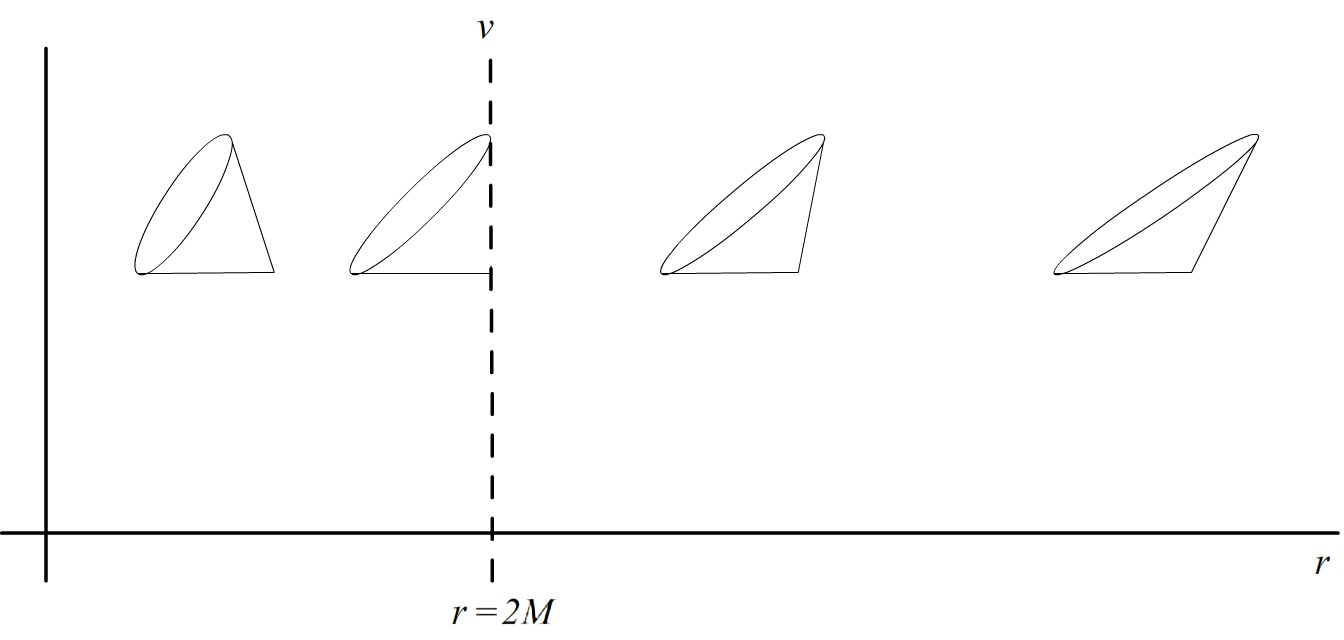
\includegraphics[scale=0.75] {fig2.jpg}
%\end{center}
				\end{figure}
                \tiny{
                $$ \frac{dv}{dr} = \left\lbrace 
            		\begin{array}{c} 0\\
						\frac{2}{1 - \frac{2M}{r}}
					\end{array} \right. $$}
			\end{center}
        \end{frame}

		
        \begin{frame}{Causal Structure in the Ingoing Eddington-Finkelstein Coordinates}
        	\begin{center}
				\begin{figure}
%\begin{center}
				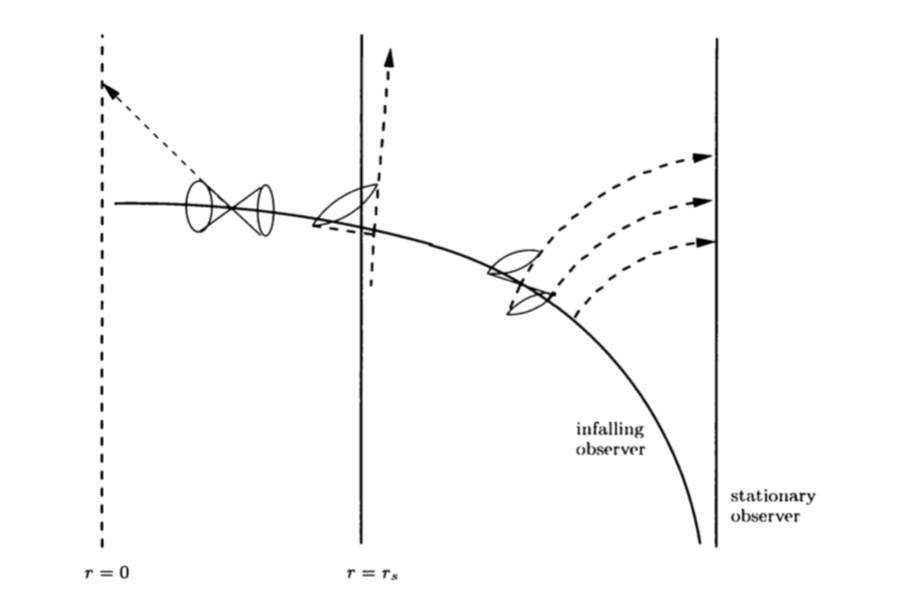
\includegraphics[scale=0.25] {fig2a.jpg}
%\end{center}
				\end{figure}
                \tiny{
                $$ \frac{dv}{dr} = \left\lbrace 
            		\begin{array}{c} 0\\
						\frac{2}{1 - \frac{2M}{r}}
					\end{array} \right. $$}
			\end{center}
        \end{frame}
  
  \begin{darkframes}        

		\begin{frame}{Outgoing Eddington-Finkelstein Coordinates}
        	$$ (t, r, \theta, \phi) \longrightarrow (u, r, \theta, \phi) $$
            \pause
            $$ u = t - r^* $$
            \pause
        	$$ r^{*} = r + 2M \ln\left| \frac{r-2M}{2M}\right| $$
            \pause
            \bigskip
            
            $$ ds^2 = -\left( 1 - \frac{2M}{r} \right) du^2 
            - 2dudr + r^2 d\Omega^2 $$
    	\end{frame}
        
        \begin{frame}{Outgoing Eddington-Finkelstein Coordinates}
            $$ ds^2 = -\left( 1 - \frac{2M}{r} \right) du^2 
            - 2dudr + r^2 d\Omega^2 $$
            \pause
            \bigskip
            While the original coordinate $r$ takes values in the range $2M < r < \infty$,
the new coordinate takes values in the range $ -\infty < u < \infty$.
    	\end{frame}
        
        \begin{frame}{Outgoing Eddington-Finkelstein Coordinates}
            $$ ds^2 = -\left( 1 - \frac{2M}{r} \right) du^2 
            - 2dudr + r^2 d\Omega^2 $$
            \pause
            \bigskip
            
            \centering
            {In these coordinates there is no singularity at $ r = 2M $.}
    	\end{frame}
        
        \begin{frame}{Causal Structure in Outgoing Eddington-Finkelstein Coordinates}
            Ingoing radial light rays move according to the conditions
            \begin{align*}
            	ds^2 &= 0\\ 
            	d\Omega &= 0
            \end{align*}
            \pause
            \bigskip
            
            $$ \frac{du}{dr} = \left\lbrace 
            		\begin{array}{c} 0\\
						- \frac{2}{1 - \frac{2M}{r}}
					\end{array} \right. $$
    	\end{frame}  
  \end{darkframes}    
  
        \begin{frame}{Causal Structure in the Outgoing Eddington-Finkelstein Coordinates}
        	\begin{center}
				\begin{figure}
%\begin{center}
				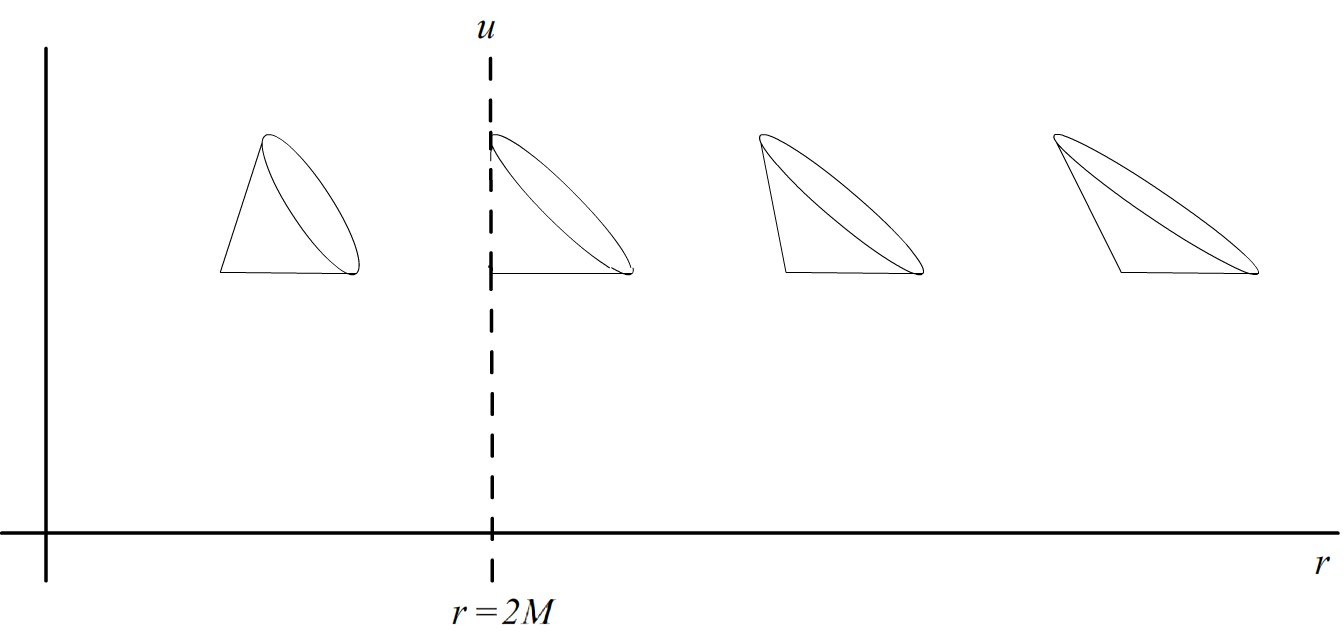
\includegraphics[scale=0.75] {fig3.jpg}
%\end{center}
				\end{figure}
                \tiny{
                $$ \frac{du}{dr} = \left\lbrace 
            		\begin{array}{c} 0\\
						-\frac{2}{1 - \frac{2M}{r}}
					\end{array} \right. $$}
			\end{center}
        \end{frame}
        
  \begin{darkframes} 
  		\begin{frame}{Next Lecture}
        	\Large
			{03. Penrose Diagrams, Hypersurfaces and Horizons}
		\end{frame}
  
  
  \end{darkframes}
\end{document}
